
\documentclass[10pt,twoside,a4paper]{article}

%%%%%%%%%%%%%%%%%%%%%%%%%%%%%%%%%%%%%%%%%%%%%%%%%%%%%%%%%%%%%%%%%%%%%%%%%%%%%%%%%%%%%%%%%%%%%%%%%%%%%%%%%%%%%%%%%%%%%%%%%%%%
\hyphenation{iSOBRAEP procedures directly papers}
\usepackage{amsmath}
\usepackage{sobraep_00,epsfig,subfigure,cite}
\usepackage{ccaption}
\usepackage[english]{babel}
\usepackage{fancyhdr}
\usepackage{times}
\usepackage{float}
\hyphenchar\font=-1

\usepackage{epstopdf}

%TCIDATA{OutputFilter=LATEX.DLL}
%TCIDATA{Created=Mon Feb 10 15:01:39 2003}
%TCIDATA{LastRevised=Tue Aug 23 19:04:24 2005}
%TCIDATA{<META NAME="GraphicsSave" CONTENT="32">}
%TCIDATA{<META NAME="DocumentShell" CONTENT="General\Blank Document">}
%TCIDATA{CSTFile=LaTeX article (bright).cst}
%TCIDATA{PageSetup=51,34,71,71,1}
%TCIDATA{Counters=arabic,1}
%TCIDATA{AllPages=
%H=36
%F=36
%}


\newtheorem{theorem}{Theorem}
\newtheorem{acknowledgement}[theorem]{Acknowledgement}
\newtheorem{algorithm}[theorem]{Algorithm}
\newtheorem{axiom}[theorem]{Axiom}
\newtheorem{case}[theorem]{Case}
\newtheorem{claim}[theorem]{Claim}
\newtheorem{conclusion}[theorem]{Conclusion}
\newtheorem{condition}[theorem]{Condition}
\newtheorem{conjecture}[theorem]{Conjecture}
\newtheorem{corollary}[theorem]{Corollary}
\newtheorem{criterion}[theorem]{Criterion}
\newtheorem{definition}[theorem]{Definition}
\newtheorem{example}[theorem]{Example}
\newtheorem{exercise}[theorem]{Exercise}
\newtheorem{lemma}[theorem]{Lemma}
\newtheorem{notation}[theorem]{Notation}
\newtheorem{problem}[theorem]{Problem}
\newtheorem{proposition}[theorem]{Proposition}
\newtheorem{remark}[theorem]{Remark}
\newtheorem{solution}[theorem]{Solution}
\newtheorem{summary}[theorem]{Summary}
\newenvironment{proof}[1][Proof]{\textbf{#1.} }{\ \rule{0.5em}{0.5em}}
\input{tcilatex}
\pagestyle{fancyplain} \thispagestyle{fancyplain} \cfoot{}
%\rfoot[\fancyplain{}{\footnotesize \sffamily\bfseries \thepage
%\hfill Eletr\^{o}nica de Pot\^{e}ncia - Vol. XX, no. X, Janeiro
%2003 }]{\fancyplain{}{}}
%\lfoot[\fancyplain{}{}]%
%{\fancyplain{}{\footnotesize \sffamily\bfseries  Eletr\^{o}nica de
%Pot\^{e}ncia - Vol. XX, no. X, Janeiro 2003 \hfill \thepage }}
\rhead{}
\lhead{}
\renewcommand{\headrulewidth}{0pt}
%\renewcommand{\footrulewidth}{0pt}
\setcounter{page}{1}




\begin{document}



\title{\textbf{COBEP - GUIDELINES FOR PUBLICATION - TITLE HERE \\(14 PT TYPE SIZE, UPPERCASE, BOLD, CENTERED)}}


\author{Author’s Names (12 pt type size, upper and lower cases, centered under the title)
\\\normalsize Author Information entered here (10 pt type size, upper and lower case, centered under the title): Affiliation)
\\\normalsize Address
\\\normalsize author@e-mail}
\maketitle

%\textbf{\textit{Abstract -- }
\begin{abstracttext}
 The authors should use these guidelines for preparing their paper. Additional information about procedures and guidelines for publication can be obtained directly with the chairman, or, through the web site iSOBRAEP: http://www.dee.feis.unesp.br/lep/revista. The papers must be submitted to COBEP only in English. This text was written according to these guidelines.
\end{abstracttext} 


\vspace{10pt} \emph{\textbf{\textit{Keywords -- }}}\textbf{The author shall provide a maximum of 6 keywords (in alphabetical order) to help identify the major topics of the paper.}

\section{INTRODUCTION}

Clearly explain the nature of the problem, previous work, purpose, and contribution of the paper.

Authors must submit their papers electronically on the web to http://www.dee.feis.unesp.br/lep/revista. From this entry page, access can be obtained to all information required for the submission. It should be noted that papers must be submitted as a PDF document. The strong requirement for publication of the accepted paper is: 

- Electronic version of the manuscript prepared in agreement with the COBEP style-file (COBEP Guidelines for publication).

\section{BODY OF THE PAPER}

This document may be used as a template for preparing your technical manuscript. Tables and Graphs: Minimum of 8 pt type size, minimum of line thickness at 0.013” or 0.30 mm, all captions should be upper and lower case, centered over 1 or 2 columns of body text.

Table \ref{table:TableI} summarizes the style and the size of the characters used in the sections of the paper.

\subsection{Pages Format }

The paper size should be A4. Top and bottom margins should be fixed to 25 mm, left margin to 18 mm and right margin to 12 mm. Rows width equal to 87 mm spaced from each other to 6 mm. Paragraph tabulation should be fixed to 4mm.

The paper is limited to no less than five pages and no more than eight pages, in a two column format.

1) Figures and tables - Figure axes labels are often a source of confusion. Try to use words rather than symbols. As an example, write the quantity "Magnetization," or "Magnetization, M," not just "M." Put units in parentheses. Do not label axes only with units. As in Figure 1, write "Magnetization (kA/m)" or "Magnetization (kA•m-1)," not just "kA/m." Do not label axes with a ratio of quantities and units. For example, write "Temperature (K)," not "Temperature/K." Figure labels should be legible, approximately 8 to 10 point type.


It should be noticed that SI (MKS) units are strongly recommended.

Large figures and tables may span both columns, but may not extend into the page margins. Figure captions should be below the figures; table captions should be above the tables. Do not put captions in "text boxes" linked to the figures. Do not put borders around your figures.

Avoid placing figures and tables before their first mention in the text.

\begin{figure}[H]
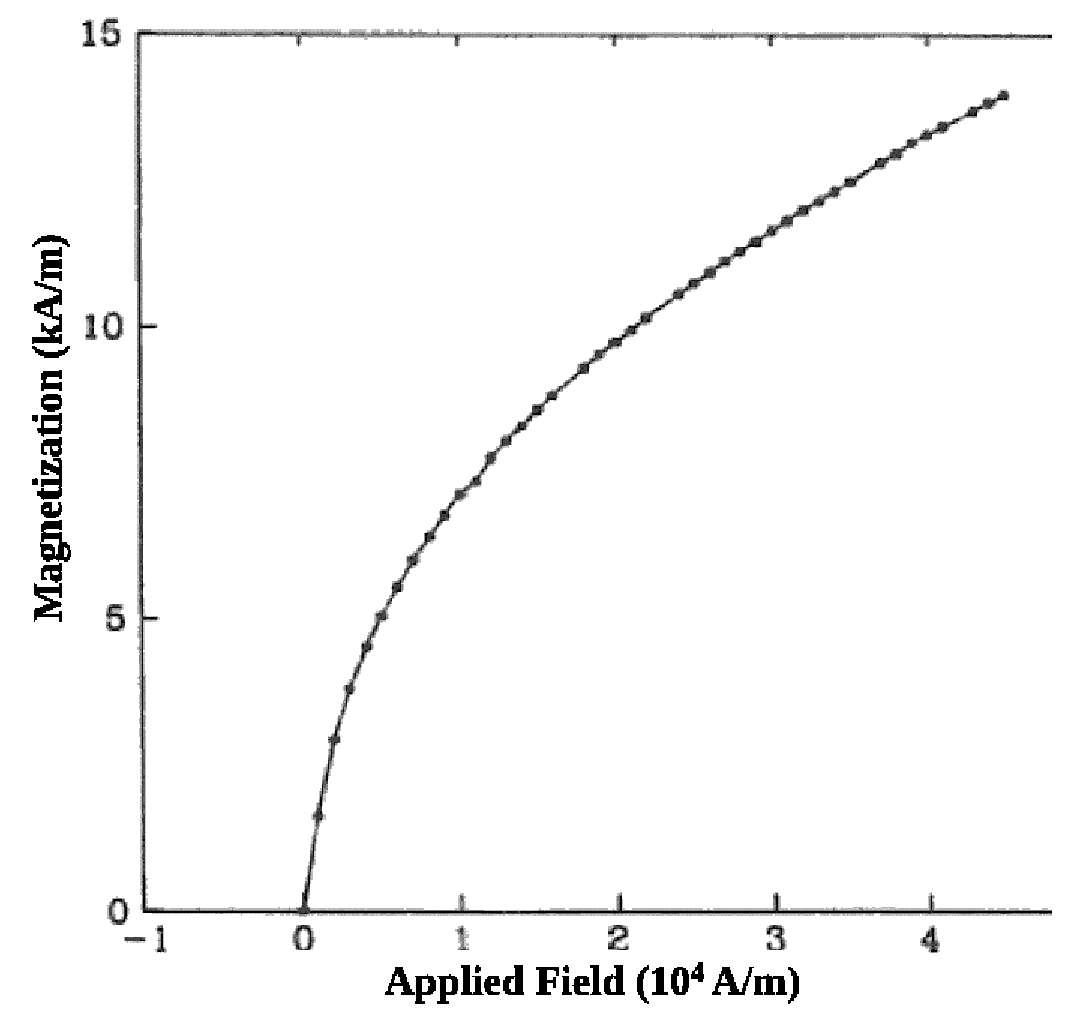
\includegraphics[angle=0,width=75mm]{figuraeng.eps}
\centering
\captiondelim{}
\captionstyle{\small\centering}
\caption{  Magnetization as a function of applied field. (Note that "Fig." is abbreviated and there is a period after the figure number followed by two spaces.)}
\par
\vspace{-.5cm}
\label{fig:fig1}
\end{figure}


\begin{table}[H]
\renewcommand{\arraystretch}{1.1}
\centering
\captiondelim{}
\captionstyle{\\}
\caption{ \textbf{Size of used characters}}
\scriptsize
\setlength{\tabcolsep}{8pt}
\begin{center}
% use packages: array
\begin{tabular}{p{0.5cm}p{2cm}p{1.5cm}p{2cm}}
\hline
\cline{1-4} 
\multicolumn{4}{c}{\textbf{Style}} \\
\hline
\textbf{Size (Points)} & \textbf{Normal} & \textbf{Bold} & \textbf{Italic} \\ 
\hline
8 & Table texts & × & × \\ 
\hline
9 & Figure captions & × & × \\ 
\hline
10 & Author information and text body & Table text & Abstract, index terms and subtitle \\ 
\hline
12 & Abstract, index terms and subtitles & × & × \\ 
\hline
14 & × & Paper title & ×\\
\hline
\cline{1-4} 
\end{tabular}\label{table:TableI}
\end{center}
\end{table}

%COLOCAR A TABELA

Illustrations and Photographs: Halftones, minimum of 8 pt type size, captions should be in upper and lower case, centered over 1 or 2 columns of body text. Images must be computer-designed and submitted as EMBEDDED images in your document. Digitized photographs in 256 grayscale are recommended.
\subsection{Equations}

Number equations consecutively with numbers in parentheses flush with the right margin, as in (1). The equation should be centered in the column and compact. Use parentheses to avoid ambiguities in denominators.

Be sure that the symbols in your equation have been defined before the equation appears or immediately following. Italicize symbols (T might refer to temperature, but T is the unit Tesla). Refer to “(1),” not “Eq. (1)” or “equation (1),” except at the beginning of a sentence: “Equation (1) is ... .”

\begin{equation}
\Delta I_{L}=I_{o}+\frac{\sqrt{3}}{2}.\frac{V_{i}}{Z}
\end{equation}
\newline
\newline
Where:

\begin{enumerate}
\item[$\Delta I_{L}$]  - Peak value of resonant current.

\item[$I_{o}$]  - Load current.

\item[$V_{i}$]  - Input voltage.
\newpage 
\item[$Z$]  - Characteristic impedance of the resonant circuit.
\end{enumerate}

\section{CONCLUSION}

A conclusion might elaborate on the importance of the work or suggest applications and extensions. Clearly indicate advantages, limitations and possible applications.

\section*{ACKNOWLEDGEMENT}

A brief acknowledgement section may be included here.

\nocite{refbib1,refbib2,refbib3}
\bibliographystyle{unsrt}
\bibliography{refbib}



\end{document}
